\documentclass[11pt]{article}
\usepackage{geometry}                % See geometry.pdf to learn the layout options. There are lots.
\geometry{letterpaper}                   % ... or a4paper or a5paper or ... 
%\geometry{landscape}                % Activate for for rotated page geometry
\usepackage[parfill]{parskip}    % Activate to begin paragraphs with an empty line rather than an indent
\usepackage{graphicx}
\usepackage{amssymb}
\usepackage{epstopdf}
\DeclareGraphicsRule{.tif}{png}{.png}{`convert #1 `dirname #1`/`basename #1 .tif`.png}

\title{GLNumericalModelingKit Optimizer}
\author{Jeffrey J. Early}
%\date{}                                           % Activate to display a given date or no date

\begin{document}
\maketitle

\section{Introduction}

Each time an operation is created it does a number of sanity checks including checking the dimensions of the variable(s) being operated on and anything else to ensure that operation is doing something that makes sense. In addition, each operation creates a new variable to store the result. All of this extra overhead is what makes GLNumericalModelingKit so nice to use because it does all the tedious bookkeeping. However, all this extra overhead also comes at a cost---creating new objects, checking dimensions, and anything else that might be happening behind the scenes can create a substantial performance penalty for code that we'd like to run very fast. GLNumericalModelingKit has an optimizer that strips out all the overhead code and automatically parallelizes operations.

One common use case for numerical modeling time-stepping forward an initial value problem of the form,
\begin{equation}
\label{ivp}
\frac{dy}{dt} = f(y).
\end{equation}
More generally $f$ is a function of $t$ as well, but we'll ignore that case for now. Note that $f$ is just a series of operations, like addition, derivatives, multiplications, etc., that defines the equation \ref{ivp}. When solving equation \ref{ivp} numerical, we must discretize it into finite time steps and then use some time stepping algorithm like 4th-order Runge-Kutta to advance to the next time point. This could be written as,
\begin{equation}
\label{timestepfunction}
y^{n+1} = RK4( f, y^n )
\end{equation}
where we've indicated the current time step by the superscript. The first argument of $RK4$ is a \emph{function} $f$ that doesn't doesn't change its form at each time step. The second argument, $y^n$ is a variable and will be different at each time step. Of course, a different time-stepping algorithm, like Leapfrog integration would have a similar form,
\begin{equation}
\label{timestepfunction2}
y^{n+1} = LF( f, y^n )
\end{equation}
but the details of the time-stepping would change. The important thing to note here is that once a time-stepping algorithm and $f$ are chosen, equations \ref{timestepfunction} and \ref{timestepfunction2} are just \emph{unary} operations that could be written,
\begin{equation}
\label{unaryop}
y^{n+1} = G( y^n ).
\end{equation}
Modeling equation \ref{ivp} numerically ultimately boils down to putting equation \ref{unaryop} into a for-loop in order to march the initial value problem forward. The point of the optimizer is to take a unary operation, like equation \ref{unaryop}, and make it really fast.

\section{Variable Operations}

GLVariableOperation subclasses takes either one GLVariable argument or two GLVariable arguments and return a resulting GLVariable. That is, they are either unary operations or binary operations on GLVariable instances. So, for example $y=e^x$, $y=k x$, $y=\textrm{fft}(x)$ are all unary operations. Yes, it's true that scalar multiplication $y=k x$ also takes $k$ as an argument, but it does only take one GLVariable as an argument. Binary operations include $y=a+b$, $y=a*b$ and so on. When you write this in code you would write,
\texttt{GLVariable *y = [a plus: b];}.
Behind the scenes there's lots happening before the actually multiplication operation actually occurs. Specifically,
\begin{enumerate}
\item \texttt{GLAdditionOperation} is being allocated and initialized.
\item The two input variables $a$ and $b$ are set, and checked that their dimensionality agrees.
\item A new variable, $y$ is being allocated an initialized with appropriate dimensions.
\item A block operation is created that is capable of performing the actual operation.
\end{enumerate}
At this stage of the code, unless you tell the equation to actually solve for $y$, the addition operation isn't actually computed. 

Now take a more complicated case like the Runge-Kutta time stepping algorithm represented by equation \ref{timestepfunction}. This includes a number of operations that can be depicted visually as in figure \ref{RungeKutta4Graph}. The $f()$ operation is, of course, the function that defines the initial value problem in equation \ref{ivp} and may represent only a single operation, or may represent a very complicated tree of operations. This algorithm requires the creation of at least 17 GLVariableOperation objects and the same number of GLVariable objects. If the function $f$ is say, 10 operations, then the algorithm requires at least 54 of each object type to be created and all the sanity checks that go with this. 1000 time steps would therefore result in 100,000 extra objects created and redundant sanity checks performed over and over again.

The key observation is to notice that as long as the single input to equation \ref{timestepfunction} remains the same at each time step, none of the extra sanity checks need to be performed again. This means that if we strip out those extra checks and just get down to the bare operations on the chunks of data, we should get a significant speed improvement.

\begin{figure}
\begin{center}
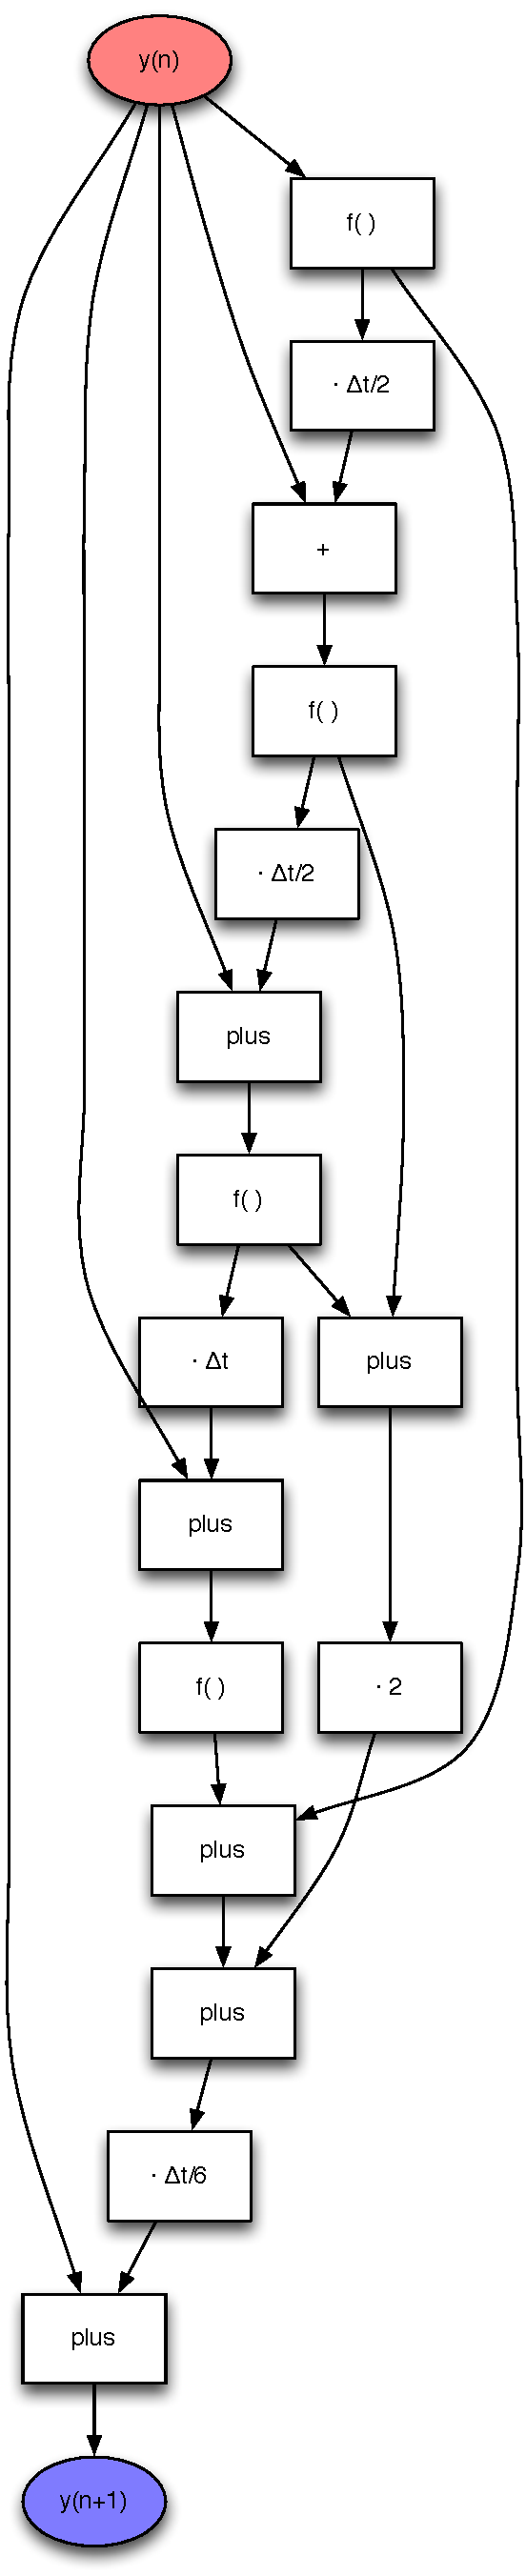
\includegraphics[width=1.6in]{RungeKutta4Graph}
\caption{Starting with variable $y$ at time step $n$ at the top in red, the fourth-order Runge-Kutta time stepping algorithm computes the variable $y$ at time step $n+1$ at the bottom in blue. The two variables are drawn as ovals, and operations are drawn as boxes. The $f()$ function is defined by the differential equation and may include several other operations.}
\label{RungeKutta4Graph}
\end{center}
\end{figure}

\section{Block Operations}

The easiest way to strip out the extra sanity checks associated with each GLVariableOperation is just string together the actual operations directly on the data. Recall the the last thing the GLAdditionOperation does is create a block operation capable of computing the actual operation. The block is created with all the necessary information it needs to be executed, like the data size or a scalar value, and can then be used as necessary.

There are currently four types of block operations that GLVariableOperations creates---unaryOperation, binaryOperation, unaryVectorOperation, and binaryVectorOperation. As the names suggest, the unaryOperation takes the result data and one operand as its arguments, while the binaryOperation takes the result data and two operands as its arguments. The unaryVectorOperation takes an array of operands and returns and an array of results which may or may not be the same size.

\begin{verbatim}
typedef void (^unaryOperation)(NSMutableData *, NSData *);
typedef void (^binaryOperation)(NSMutableData *, NSData *, NSData *);
typedef void (^unaryVectorOperation)(NSArray *, NSArray *);
typedef void (^binaryVectorOperation)(NSArray *, NSArray *, NSArray *);
\end{verbatim}

Each GLVariableOperation creates the appropriate block operation and does as much computation as is possible before it needs the actual data. Some GLVariableOperations also return different blocks depending on what optimizations can be made given the input values.

The goal of the optimizer is now more concrete. The optimizer needs to take a graph of operations, like equation \ref{timestepfunction} shown in figure \ref{RungeKutta4Graph}, and string together the block operations into one larger block. In the case of equation  \ref{timestepfunction}, all the block operations can be condensed into a single unaryOperation---one operand, one result. What is perhaps also clear from figure \ref{RungeKutta4Graph}, is that many of these operations can be completed in parallel. Furthermore, the graph dependencies also allow us to deduce exactly how much memory needs to be allocated so that we can use minimal memory footprint.

\section{Algorithm Components}

Before actually considering the algorithm used to optimize the graph, it's helpful to break the graph down into the different components and establish terminology.

Consider first the the relatively complicated quasigeostrophic equation
\begin{equation}
\label{qg}
\nabla^2 \eta_t  -  \eta_t + \eta_x +  J \left( \eta, \nabla^2 \eta \right) - k \nabla^4 \eta = 0
\end{equation}
which fits the form of equation \ref{ivp} where $y=(\nabla^2 -1)\eta$ and $f= \eta_x +  J \left( \eta, \nabla^2 \eta \right) - k \nabla^4 \eta$. If we assume that we are given $y$ in the frequency domain, then the series of algebraic operations for $f(y)$ is represented by the graph in figure \ref{QGfFromY}. This graph has \emph{almost} the same properties as the graph in figure \ref{RungeKutta4Graph}, except for the addition of precomputed variables (associated with differentiation) highlighted in the green boxes.

\begin{figure}
\begin{center}
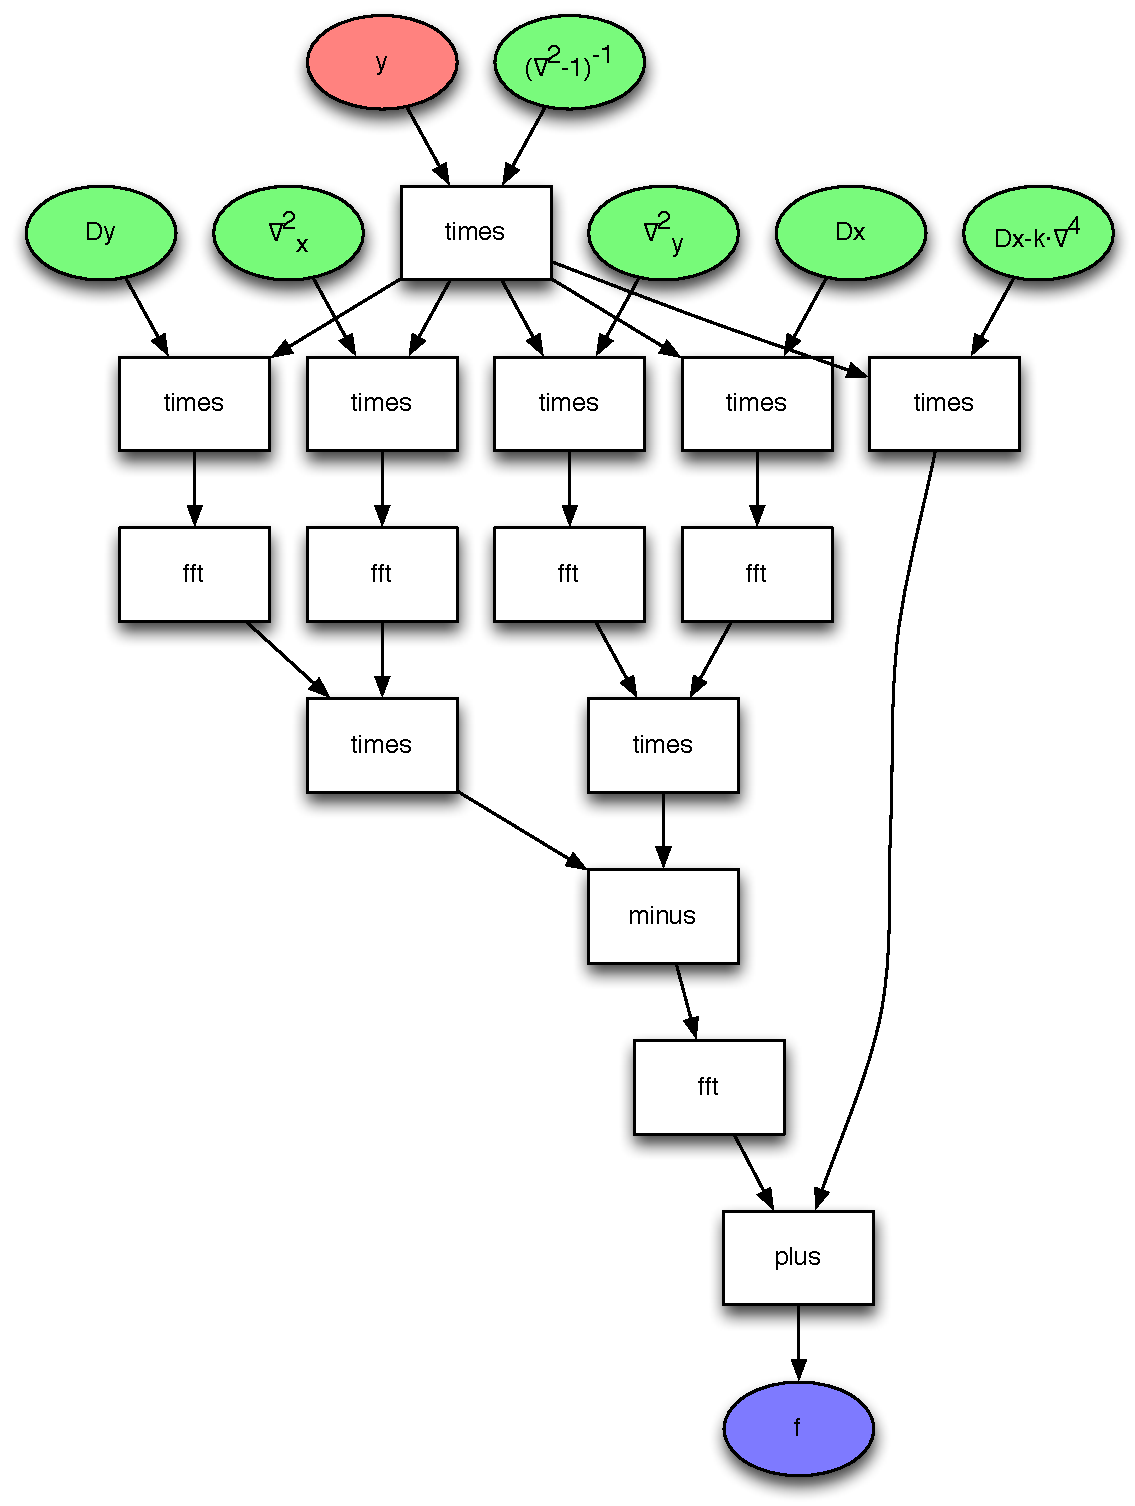
\includegraphics[width=4.8in]{QGfFromY}
\caption{Starting with the variable $y$ in the frequency domain (red), this graph shows the operations necessary to compute the variable $f$ in the frequency domain (blue) for the nonlinear quasigeostrophic equation. The green colored variables are precomputed differential operators or, more generally, constant variables used in the calculations. Variables are shown as ovals and operations are shown as boxes.}
\label{QGfFromY}
\end{center}
\end{figure}

The components of the graph are identified with the following terminology,
\begin{itemize}
\item \emph{Top variables}---the operands/input variables of the final operation. The single top variable is highlighted in red in figure \ref{QGfFromY}.
\item \emph{Bottom variable}---the result/output variables of the final operation.The single bottom variable is highlighted in blue in figure \ref{QGfFromY}.
\item \emph{Precomputed variable}---a constant variable, such as a differential operator highlighted in green in figure \ref{QGfFromY}.
\item \emph{Generated variable}---a variable whose value is to-be-determined at run-time. This could be a randomly generated variable, or one fetched from a file, based on the current time.
\item \emph{Unary operation}---an operation with one operand and one resulting variable, shown in white with a single input in figure \ref{QGfFromY}.
\item \emph{Binary operation}---an operation with two operands and one resulting variable, shown in white with two inputs in figure \ref{QGfFromY}.
\item \emph{Dependency/parent}---an incoming line, an operand. Unary operations have one dependency, binary operations have two.
\item \emph{Dependent/child}---an outgoing line. All operations have at least one dependent, but may have any number.
\end{itemize}

In order to do its job, the optimizer is given the top variables and the bottom variables. From these two variables, the optimizer is able to internally recreate the graphs of figures \ref{RungeKutta4Graph} and \ref{QGfFromY}. There are a few basic things to notice about these graphs.

\begin{enumerate}
\item Unary operations have exactly one dependency, but may have multiple dependents.
\item Binary operations have exactly two dependencies, but may have multiple dependents.
\item Some binary operations may depend on a precomputed variable.
\item Unary operations dependent on precomputed variables and binary operations dependent on two precomputed variables can always be reduced to a precomputed variable.
\item Operations with multiple dependencies can be thought of as a \emph{thread split}. That is, the dependencies can operate in parallel.
\item Binary operations (not dependent on precomputed variables) are \emph{thread joins}.
\item There are exactly as many thread splits as thread joints in a unary operation.
\end{enumerate}

In the visual representation of the operation graphs the distinction between variables and operations is made by depicting ovals and rectangles, respectively. However, the terminology and thought process can be easily blurred since each operation results in exactly one variable, which is then passed on to one or more other operations as input variables. The one-to-one correspondence between variables and operations is useful if you are careful to think of the variable as a result of completing its operation.

\section{Grand Central Dispatch}

Central to the optimizer is the use of grand central dispatch (gcd), a library designed for executing blocks. In brief, a block with no input or return values is added to a global queue to be executed.

One of the features offered by gcd is simple management of thread splits and thread joins with groups. The idea is that a you call a function to add your block to the queue as usual, but you also pass it a group. The block won't actually be added to the queue until the group's count is equal to zero. The idea being that other operations, upon which the first block depends, can decrement the group count when they have finished processing. GCD waits until the group count hits zero before actually adding the block to the queue.

The strategy taken here is to use groups to regulate when binary operations get executed. The binary operation has two dependencies/parents. One of its parents will simply decrement the group count when it's done with its computation, while the other will add the block to the queue associated with that group when it's done. It does not matter which parent does its job first.

\section{The Key Idea}

The ultimate goal of the optimizer is to create a final consolidated unaryOperation, binaryOperation, or unaryVectorOperation from a complicated graph. These final operations will get created in the last step of the algorithm after \emph{execution blocks} have been created for all of the operations. An executionBlock takes the form
\begin{verbatim}
typedef void (^executionBlock)(NSArray *);
\end{verbatim}
where the single input argument is an array of NSData objects. The array is ordered to contain the NSData objects of bottom variables, followed by the NSData objects of the top variables and finally all of the internal data buffers.

The optimizer creates an \emph{execution block} for every \emph{operation}, such as is shown in the graphs of figures \ref{RungeKutta4Graph} and \ref{QGfFromY}. The basic idea is that \textbf{each execution block is responsible for running its operation on the appropriate data buffers and then taking care of its dependents}. Let's consider both of these steps in turn.

\subsection{Operation Execution}
The first job of the executionBlock is to execute the operation it is responsible for on the appropriate data buffers. The execution block will have been created from either a unaryOperation or a binaryOperation and will therefore need to either two or three of the data buffers from the array, respectively. Because the array's order is guaranteed, the indices of the appropriate data buffers are copied by the block at the time of the blocks creation. When it comes time to run, the execution block simply grabs the appropriate data buffers and runs the operation.

\subsection{Dependents}
The execution block is also responsible for `taking care of' its dependents. This responsibility breaks down do doing one of three things for each of its dependents,
\begin{enumerate}
\item Add a dependent execution block to the queue.
\item Add a dependent execution block to the queue with a group.
\item Decrement a group count.
\end{enumerate}

The first possibility, adding a dependent execution block to the queue, means that the dependent execution block will be run immediately. This means that the dependent is either a unaryOperation (which only depends on this parent) or it's a binary operation whose other parent is precomputed or is another top variable and can therefore also be run immediately.

The second and third possibilities arise only for execution blocks created from binary operations. In this case, one parent is responsible for adding the dependent execution block to the queue associated with the group, and the other parent is responsible is responsible from decrementing the group count.

Creating these execution blocks and assigning responsibilities to the parents requires a bottom-up approach: an execution block can only be created if the execution blocks for its dependents have already been created. This means that as a first step we must create an \emph{execution plan} where the responsibilities of each execution block is tallied. In the second step, the execution blocks will be created, but only when the expected number of dependent execution blocks have been created.

\section{Execution Plan}

Consider the algorithm to decide which of the three responsibilities each parent will handle. Note that the following algorithm assumes that we can only establish if a variable is precomputed after we have established that it is not a top variable. This increases the number of if statements.

\begin{enumerate}
\item Unary operations:
\begin{enumerate}
\item if the parent is precomputed, we need to compute this now and optimize.
\item else add to the queue without a group by their only parent.
\end{enumerate}
\item Binary operation:
\begin{enumerate}
\item if parent A and B are top variables,  add to the queue without a group by parent A (no need to wait).
\item if parent A is a top variable, parent B is precomputed, add to the queue without a group by parent A (no need to wait).
\item if parent A is a top variable, add the queue with a group by parent A, parent B must exit the group upon completion.
\item if parent B is a top variable, parent A is precomputed, add to the queue without a group by parent B (no need to wait).
\item if parent B is a top variable, add the queue with a group by parent B, parent A must exit the group upon completion.
\item if parent A and B are precomputed, we need to compute this now and optimize.
\item if parent A is precomputed, add to the queue without a group by parent B (no need to wait).
\item if parent B is precomputed, add to the queue without a group by parent A (no need to wait).
\item else, add to the queue with a group by parent A, parent B must exit the group upon completion.
\end{enumerate}
\end{enumerate}

The last part of the algorithm, (2i), is arbitrary and could have A and B swapped.

Note that unaryVectorOperations and binaryVectorOperations are very similar to binaryOperations in that they may have multiple parents. The parents can be divided into three categories---top variables, precomputed variables, other variables.

\begin{enumerate}
\item if there are only precomputed variables, stop now and optimize.
\item if there are top variables and no other variables,  add to the queue without a group by a top variable parent.
\item if there are top variables and other variables, add to the queue with a group by a top variable, all other parents must exit the group.
\item if there are no top variables and only one other variable, add to the queue without a group by the other variable
\item if there are no top variables and multiple other variables, add to the queue with a group by one variable, all others must exit the group
\end{enumerate}

The last operations, upon which the bottom variables depend, have the additional responsibility that they must exit a group to indicate that they are done with their computation. This allows the final operation to know when it's finished computing.

The execution plan runs through the graph, starting from each bottom variable variable and branching at all binary operations, and simply tallies up how many of the three types of operations each execution block will be responsible for.

After the execution plan is created, the memory plan can be created. The algorithm to create the execution blocks is subsequently run, also from the bottom up, and an execution block is created when the total number of expected dependents/child execution blocks are ready.

\section{Memory Plan}

April 25 

The input and output variables of the final operation are variable memory addresses. For example, a unaryOperation takes two variables, the result (bottom) variable and the operand (top) variable. These are NSMutableData and NSData objects whose addresses are expected to change. Similarly, a final binaryOperation would take three variables, and a unaryVectorOperation would take two arrays of variables.

All the variables that are created in between the top and bottom variables just serve as internal memory buffers which we will preallocate. The most basic thing to do is simply to assign a unique NSData object to each variable. However, as operations complete, some of those buffers are free to be reused, and therefore an NSData object is not needed for each internal variable in the graph.

Another way to look at this is that that each variable can use data from variables that are both 1) reachable and 2) don't include said variable as an intermediate variable.

In the approach taken here an NSData buffer is created and then offered to one of the bottom variables (which doesn't actually need one). The variable then offers it to a parent and recursively works its way to the top of the tree.

Some basic rules and observations about memory management.
\begin{enumerate}
\item If an operation does not support in-place memory buffers, the parent cannot use the same data buffer, although a grandparent can. However, if the operation does support in-place operations, then we can simply pass the data buffer to the parent.

\item Every thread join (binary) operation has a unique thread split operation (or none at all). The thread split variable can be found by looking for the first variable reachable by all possible branches. We call this unique parent the ur parent.

\item A data buffer used by a binary operation (thread join) can only be offer to the thread split operation (somewhere up the tree), if it doesn't have a data buffer yet---otherwise, it can be offered to the parent or grandparent as usual.

\item A data buffer should be used whenever possible. So if the data buffer is offered up one branch (say the left branch) of a thread split but is not used, then it should instead be offered up the right branch.

\item You can offer an over-sized data buffer to a variable -- BUT, the variable should only take it if it doesn't interfere with a parent that might otherwise use it.

\end{enumerate}

Offer the data buffer to a variable---if we don't have one, and it's the right size, use it. How do we offer it up the tree?
\begin{enumerate}
\item If we're at a thread join/binary operation and the ur parent does want our variable, skip to the ur parent and progress
\item If we're at a thread join/binary operation and the ur parent doesn't want our variable or already has one, we can offer it straight up one branch of the tree. But which branch? We don't want to send it up the same branch each time?
\item Send it up one side of the branch and insist it doesn't traverse beyond. If it comes back with some success... then what? Start at the ur parent and continue. If it came back with no success, try the other branch. But that's stupid you see, because either side could have a divergent binary operation that goes beyond the ur parent.

\item Do we offer this to the thread split variable? If we didn't take the variable and it doesn't have one, then yes. If we did take the variable and it doesn't have one 
\item else
\begin{enumerate}
\item 
\end{enumerate}
\end{enumerate}

\begin{enumerate}

\item 

\item Alternatively, we can try to reuse those memory buffers whenever possible. If an operation does not support in-place memory buffers, we can only offer the data buffer to the grandparent. However, if the operation does support in-place operations, then we can simply pass the data buffer to the parent.

The tricky part becomes knowing when a buffer can be reused during parallel operations. If the variable has only one parent, then the buffer can be passed up to the parent (or grandparent). However, if the variable has two parents, in other words, it's a thread join, then the buffer cannot be used until we find where the threads split.

The memory allocation algorithm, similar to the execution plan, starts with the bottom most variables and works its way to the top. Bottom variables and top variables don't need buffers. Precomputed variables just get copied, but their data buffers can't be used later in the computation because the precomputed value will be needed again for the next time the operation is called. All other variables not already assigned a data buffer, create a new buffer. However, before continuing, that variable offers the data buffer to its grandparents. The grandparents variable use that data buffer if its the right size and they don't already have one, and then offer it to \emph{their} grandparents. If the grandparents don't use the data buffer, its offered to the parents. The offering continue up the chain until a top or precomputed variable is reached. The only exception is that binary operations offer the variable up the first operand branch, and only if it wasn't used by any parent on that branch is is it offered up the second branch.

For an RK4 time stepping the QG equation plus a tracer, this reduced the memory requirements from 138 buffers to 87 buffers.

\item Finally, but asking each operation whether it supports in-place memory buffers or not, we can optimize this even further. I

For an RK4 time stepping the QG equation plus a tracer, this reduced the memory requirements down to 71 buffers---almost half of the original, simplest algorithm.

\end{enumerate}

\section{Execution Block Creation}

The algorithm to create the execution blocks is subsequently run, from the bottom up, and an execution block is created when the total number of expected dependents/child execution blocks are ready. Creation of the top most block (the desired unaryOperation, binaryOperation or unaryVectorOperation) is punted until later.

Starting from the bottom variables, the algorithm asks for an execution block to be created for a given variable. The bottom variables, of course, have no dependents and can therefore be created immediately. Following the identical algorithm as in the execution plan, the resulting execution block is handed to the appropriate parent. Often a variable will be reached that does not have the expected number of responsibilities created yet. This will occur because not all the branches of the tree reaching that variable have been traversed yet. For this reason, the tree traversal algorithm will need to be called multiple times until all of the execution blocks are created.

\section{Final Block Creation}

Once all of the execution blocks have been created, it is then possible to construct the final unaryOperation, binaryOperation, or unaryVectorOperation block. This final block is responsible for handling all the execution blocks associated with the top variables, but also has two additional responsibilities. First, it must create the array of data buffers from its input arguments and the internal buffers that gets passed down to all of the execution blocks. Second, it must enter all the groups that will later be exited by its dependents (including the execution blocks associated with the bottom variables).

\section{New Algorithm}

The core algorithm for treating dependencies remains the same. However, some changes to the final block creation and variable storage have been changed.

The new key idea is that the optimizer creates a GLVariableOperation subclass, which can be used over and over again.

There are five types of variables that the optimizer has to manage. Note that the first four types require a buffer in one-to-one correspondence with a variable, whereas the last type requires a group of buffers in correspondence with an operation.
\begin{enumerate}
\item TopVariables will become the operands of the optimized operation. They are copied (without data) and stored so that they can be compared to future input.
\item BottomVariables will become the results of the optimized operation. They are copied (without data) and stored so that they can be used for future output.
\item PrecomputedVariables will have their data copied so they can be used directly in the optimized operation block.
\item InternalVariables will become buffers in the optimized operation, so they do not need to be retained, although their size will need to be captured.
\item InternalBuffers will remain buffers in the optimized operations, so they also do not need to be retained.
\end{enumerate}


\end{document}  